\section{Software}

The submarine's software is aware of the competition objectives, and performs computer vision to
command the submarine to move through the embedded system.
The computer vision uses the OpenCV library to help identify objects based on shape and color.
The video input consists of two webcams, one facing forward and one facing down.
These cameras are rigidly attached to the AUV, and the AUV must move to change the viewpoint.
The software also includes a graphical simulator that we can use to test our computer vision algorithms.

\subsection{Software Organization}
\label{gui}


\begin{figure}
\begin{center}
 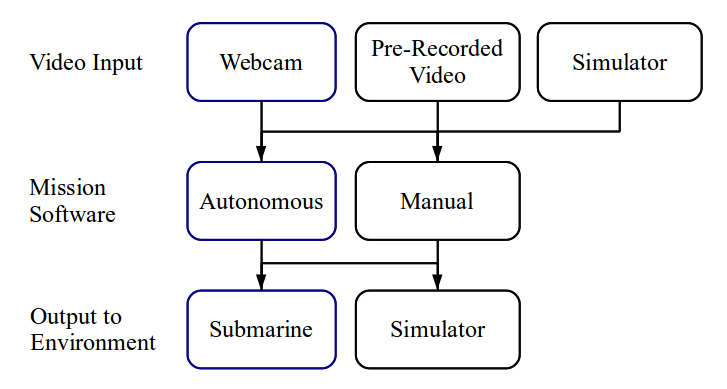
\includegraphics[height=1.9in]{fig/modules.png}
\caption{Software module organization.}\label{vision}
\end{center}
\end{figure}


\begin{figure}
\begin{center}
 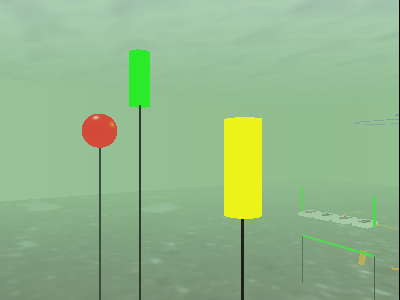
\includegraphics[height=1.9in]{fig/sim.png}
\caption{Example image from the simulator showing pipe segments and the buoys
         in turbid water.}\label{sim}
\end{center}
\end{figure}

The software is broken down into 3
components (Figure~\ref{vision}): (i) the video input;
(ii) the mission software gives physical commands to move the sub;
and (iii) the environment that reacts to the physical commands.
The video input can come from the submarine's webcams, pre-recorded video,
or the simulator (Figure~\ref{sim}). The mission software can be the autonomous
algorithms that drive the submarine or a manually controlled user interface.
The environment that reacts to physical commands can be the submarine or the
simulator. The different permutations to hook up the software components
solely created to test and debug the vision
algorithms when AquaTux is not functioning autonomously.
These software interfaces help ensure the software to test the submarine
resembles the autonomous functionality as much as possible.
The manual user interface allows us to act as a passive observer,
constantly requesting the state of the vehicle,
or as a controller sending commands to the AUV.


\vspace{-.1in}
\subsection{Image Processing Software}
The image processing software consists of color filters and edge and
line detection algorithms. The color filters allow us to select
specific information to only process relevant parts of the images. The
line processing algorithms use heuristics to form polygons and
recognize objects such as pipes or boxes, that have a well defined
appearance. Our algorithms are robust enough to recognize objects even
if their view changes due to perspective or the presence of debris in
the water.  The mission software consists of a main loop that acquires
images, processes them and send commands to the other subsystems on
one of the two serial ports of the embedded computer (see
Section~\ref{gui}).

The mission is broken down into modular tasks that
can me chained or tested individually. Tasks proceed by first
identifying a target for the vehicle to begin pursuit. If the object
in question is not found, the vehicle rotates on its vertical axis
(yaw) to make the cameras pan to the right and to the left. If nothing
is found, then the vehicle proceeds forward in its initial direction.
Once a target is acquired, the vertical position and lateral positions
of the vessel are controlled to match the desired coordinates.  The
vehicle uses a combination of heading relative to its current
orientation and absolute headings (relative to the magnetic north
pole) to navigate inside the environment. This alleviates the need to
get real-time measurements of the heading as the vehicle is
navigating. A limitation of our vision hardware that we had to address
is to determine when a task is completed if the view of the target is
obscured or occluded due to the AUV's proximity (e.g. it is passing
under the gate). In such situations, for the moment being, we use
timers to ensure that the vehicle reaches its target location.
